% Created by tikzDevice version 0.12.3 on 2019-09-26 18:26:44
% !TEX encoding = UTF-8 Unicode
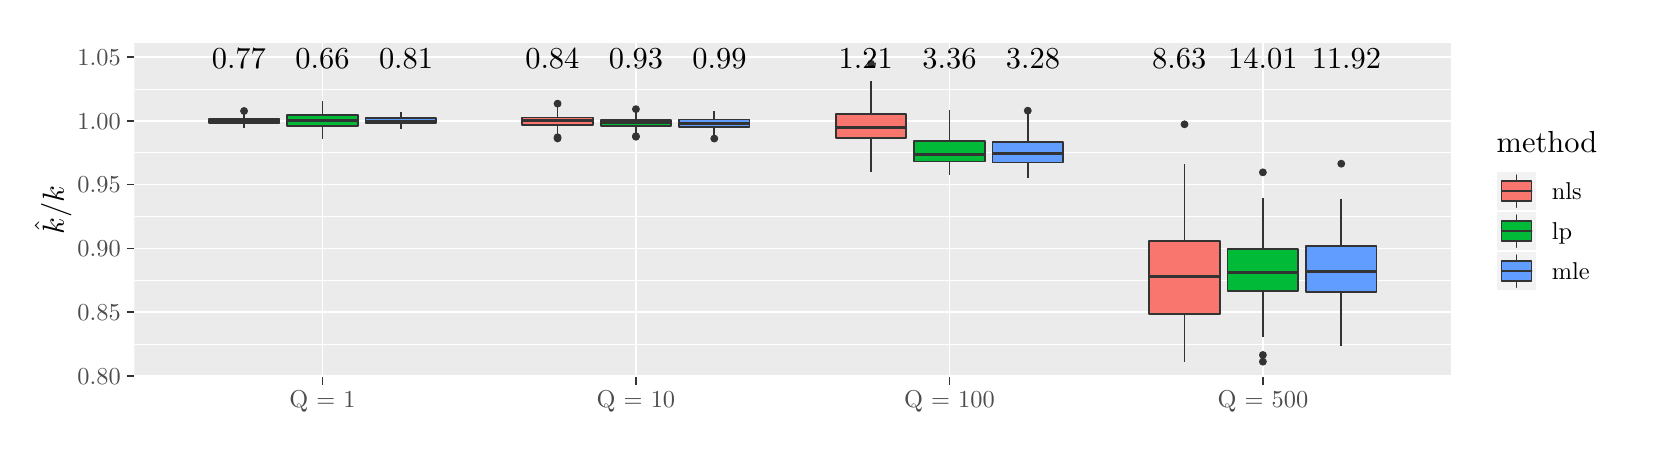
\begin{tikzpicture}[x=1pt,y=1pt]
\definecolor{fillColor}{RGB}{255,255,255}
\path[use as bounding box,fill=fillColor,fill opacity=0.00] (0,0) rectangle (578.16,144.54);
\begin{scope}
\path[clip] (  0.00,  0.00) rectangle (578.16,144.54);
\definecolor{drawColor}{RGB}{255,255,255}
\definecolor{fillColor}{RGB}{255,255,255}

\path[draw=drawColor,line width= 0.6pt,line join=round,line cap=round,fill=fillColor] (  0.00,  0.00) rectangle (578.16,144.54);
\end{scope}
\begin{scope}
\path[clip] ( 38.56, 18.22) rectangle (514.31,139.04);
\definecolor{fillColor}{gray}{0.92}

\path[fill=fillColor] ( 38.56, 18.22) rectangle (514.31,139.04);
\definecolor{drawColor}{RGB}{255,255,255}

\path[draw=drawColor,line width= 0.3pt,line join=round] ( 38.56, 30.23) --
	(514.31, 30.23);

\path[draw=drawColor,line width= 0.3pt,line join=round] ( 38.56, 53.27) --
	(514.31, 53.27);

\path[draw=drawColor,line width= 0.3pt,line join=round] ( 38.56, 76.31) --
	(514.31, 76.31);

\path[draw=drawColor,line width= 0.3pt,line join=round] ( 38.56, 99.35) --
	(514.31, 99.35);

\path[draw=drawColor,line width= 0.3pt,line join=round] ( 38.56,122.39) --
	(514.31,122.39);

\path[draw=drawColor,line width= 0.6pt,line join=round] ( 38.56, 18.71) --
	(514.31, 18.71);

\path[draw=drawColor,line width= 0.6pt,line join=round] ( 38.56, 41.75) --
	(514.31, 41.75);

\path[draw=drawColor,line width= 0.6pt,line join=round] ( 38.56, 64.79) --
	(514.31, 64.79);

\path[draw=drawColor,line width= 0.6pt,line join=round] ( 38.56, 87.83) --
	(514.31, 87.83);

\path[draw=drawColor,line width= 0.6pt,line join=round] ( 38.56,110.87) --
	(514.31,110.87);

\path[draw=drawColor,line width= 0.6pt,line join=round] ( 38.56,133.91) --
	(514.31,133.91);

\path[draw=drawColor,line width= 0.6pt,line join=round] (106.52, 18.22) --
	(106.52,139.04);

\path[draw=drawColor,line width= 0.6pt,line join=round] (219.79, 18.22) --
	(219.79,139.04);

\path[draw=drawColor,line width= 0.6pt,line join=round] (333.07, 18.22) --
	(333.07,139.04);

\path[draw=drawColor,line width= 0.6pt,line join=round] (446.34, 18.22) --
	(446.34,139.04);
\definecolor{drawColor}{gray}{0.20}
\definecolor{fillColor}{gray}{0.20}

\path[draw=drawColor,line width= 0.4pt,line join=round,line cap=round,fill=fillColor] ( 78.20,114.43) circle (  1.21);

\path[draw=drawColor,line width= 0.6pt,line join=round] ( 78.20,111.51) -- ( 78.20,113.47);

\path[draw=drawColor,line width= 0.6pt,line join=round] ( 78.20,110.18) -- ( 78.20,108.34);
\definecolor{fillColor}{RGB}{248,118,109}

\path[draw=drawColor,line width= 0.6pt,line join=round,line cap=round,fill=fillColor] ( 65.46,111.51) --
	( 65.46,110.18) --
	( 90.94,110.18) --
	( 90.94,111.51) --
	( 65.46,111.51) --
	cycle;

\path[draw=drawColor,line width= 1.1pt,line join=round] ( 65.46,110.82) -- ( 90.94,110.82);

\path[draw=drawColor,line width= 0.6pt,line join=round] (106.52,113.10) -- (106.52,118.19);

\path[draw=drawColor,line width= 0.6pt,line join=round] (106.52,109.07) -- (106.52,104.19);
\definecolor{fillColor}{RGB}{0,186,56}

\path[draw=drawColor,line width= 0.6pt,line join=round,line cap=round,fill=fillColor] ( 93.78,113.10) --
	( 93.78,109.07) --
	(119.26,109.07) --
	(119.26,113.10) --
	( 93.78,113.10) --
	cycle;

\path[draw=drawColor,line width= 1.1pt,line join=round] ( 93.78,110.93) -- (119.26,110.93);

\path[draw=drawColor,line width= 0.6pt,line join=round] (134.84,111.78) -- (134.84,114.21);

\path[draw=drawColor,line width= 0.6pt,line join=round] (134.84,110.13) -- (134.84,107.88);
\definecolor{fillColor}{RGB}{97,156,255}

\path[draw=drawColor,line width= 0.6pt,line join=round,line cap=round,fill=fillColor] (122.09,111.78) --
	(122.09,110.13) --
	(147.58,110.13) --
	(147.58,111.78) --
	(122.09,111.78) --
	cycle;

\path[draw=drawColor,line width= 1.1pt,line join=round] (122.09,110.74) -- (147.58,110.74);
\definecolor{fillColor}{gray}{0.20}

\path[draw=drawColor,line width= 0.4pt,line join=round,line cap=round,fill=fillColor] (191.48,104.94) circle (  1.21);

\path[draw=drawColor,line width= 0.4pt,line join=round,line cap=round,fill=fillColor] (191.48,104.51) circle (  1.21);

\path[draw=drawColor,line width= 0.4pt,line join=round,line cap=round,fill=fillColor] (191.48,117.09) circle (  1.21);

\path[draw=drawColor,line width= 0.6pt,line join=round] (191.48,112.13) -- (191.48,116.22);

\path[draw=drawColor,line width= 0.6pt,line join=round] (191.48,109.38) -- (191.48,106.01);
\definecolor{fillColor}{RGB}{248,118,109}

\path[draw=drawColor,line width= 0.6pt,line join=round,line cap=round,fill=fillColor] (178.73,112.13) --
	(178.73,109.38) --
	(204.22,109.38) --
	(204.22,112.13) --
	(178.73,112.13) --
	cycle;

\path[draw=drawColor,line width= 1.1pt,line join=round] (178.73,110.85) -- (204.22,110.85);
\definecolor{fillColor}{gray}{0.20}

\path[draw=drawColor,line width= 0.4pt,line join=round,line cap=round,fill=fillColor] (219.79,105.14) circle (  1.21);

\path[draw=drawColor,line width= 0.4pt,line join=round,line cap=round,fill=fillColor] (219.79,115.10) circle (  1.21);

\path[draw=drawColor,line width= 0.4pt,line join=round,line cap=round,fill=fillColor] (219.79,105.31) circle (  1.21);

\path[draw=drawColor,line width= 0.6pt,line join=round] (219.79,111.26) -- (219.79,114.10);

\path[draw=drawColor,line width= 0.6pt,line join=round] (219.79,108.94) -- (219.79,105.66);
\definecolor{fillColor}{RGB}{0,186,56}

\path[draw=drawColor,line width= 0.6pt,line join=round,line cap=round,fill=fillColor] (207.05,111.26) --
	(207.05,108.94) --
	(232.54,108.94) --
	(232.54,111.26) --
	(207.05,111.26) --
	cycle;

\path[draw=drawColor,line width= 1.1pt,line join=round] (207.05,110.11) -- (232.54,110.11);
\definecolor{fillColor}{gray}{0.20}

\path[draw=drawColor,line width= 0.4pt,line join=round,line cap=round,fill=fillColor] (248.11,104.47) circle (  1.21);

\path[draw=drawColor,line width= 0.6pt,line join=round] (248.11,111.30) -- (248.11,114.33);

\path[draw=drawColor,line width= 0.6pt,line join=round] (248.11,108.65) -- (248.11,104.77);
\definecolor{fillColor}{RGB}{97,156,255}

\path[draw=drawColor,line width= 0.6pt,line join=round,line cap=round,fill=fillColor] (235.37,111.30) --
	(235.37,108.65) --
	(260.86,108.65) --
	(260.86,111.30) --
	(235.37,111.30) --
	cycle;

\path[draw=drawColor,line width= 1.1pt,line join=round] (235.37,109.96) -- (260.86,109.96);
\definecolor{fillColor}{gray}{0.20}

\path[draw=drawColor,line width= 0.4pt,line join=round,line cap=round,fill=fillColor] (304.75,131.49) circle (  1.21);

\path[draw=drawColor,line width= 0.6pt,line join=round] (304.75,113.36) -- (304.75,125.29);

\path[draw=drawColor,line width= 0.6pt,line join=round] (304.75,104.56) -- (304.75, 92.33);
\definecolor{fillColor}{RGB}{248,118,109}

\path[draw=drawColor,line width= 0.6pt,line join=round,line cap=round,fill=fillColor] (292.01,113.36) --
	(292.01,104.56) --
	(317.49,104.56) --
	(317.49,113.36) --
	(292.01,113.36) --
	cycle;

\path[draw=drawColor,line width= 1.1pt,line join=round] (292.01,108.63) -- (317.49,108.63);

\path[draw=drawColor,line width= 0.6pt,line join=round] (333.07,103.66) -- (333.07,114.69);

\path[draw=drawColor,line width= 0.6pt,line join=round] (333.07, 96.18) -- (333.07, 91.17);
\definecolor{fillColor}{RGB}{0,186,56}

\path[draw=drawColor,line width= 0.6pt,line join=round,line cap=round,fill=fillColor] (320.33,103.66) --
	(320.33, 96.18) --
	(345.81, 96.18) --
	(345.81,103.66) --
	(320.33,103.66) --
	cycle;

\path[draw=drawColor,line width= 1.1pt,line join=round] (320.33, 98.85) -- (345.81, 98.85);
\definecolor{fillColor}{gray}{0.20}

\path[draw=drawColor,line width= 0.4pt,line join=round,line cap=round,fill=fillColor] (361.39,114.54) circle (  1.21);

\path[draw=drawColor,line width= 0.6pt,line join=round] (361.39,103.12) -- (361.39,113.89);

\path[draw=drawColor,line width= 0.6pt,line join=round] (361.39, 95.86) -- (361.39, 90.16);
\definecolor{fillColor}{RGB}{97,156,255}

\path[draw=drawColor,line width= 0.6pt,line join=round,line cap=round,fill=fillColor] (348.64,103.12) --
	(348.64, 95.86) --
	(374.13, 95.86) --
	(374.13,103.12) --
	(348.64,103.12) --
	cycle;

\path[draw=drawColor,line width= 1.1pt,line join=round] (348.64, 99.17) -- (374.13, 99.17);
\definecolor{fillColor}{gray}{0.20}

\path[draw=drawColor,line width= 0.4pt,line join=round,line cap=round,fill=fillColor] (418.02,109.62) circle (  1.21);

\path[draw=drawColor,line width= 0.6pt,line join=round] (418.02, 67.39) -- (418.02, 95.36);

\path[draw=drawColor,line width= 0.6pt,line join=round] (418.02, 41.17) -- (418.02, 23.71);
\definecolor{fillColor}{RGB}{248,118,109}

\path[draw=drawColor,line width= 0.6pt,line join=round,line cap=round,fill=fillColor] (405.28, 67.39) --
	(405.28, 41.17) --
	(430.77, 41.17) --
	(430.77, 67.39) --
	(405.28, 67.39) --
	cycle;

\path[draw=drawColor,line width= 1.1pt,line join=round] (405.28, 54.70) -- (430.77, 54.70);
\definecolor{fillColor}{gray}{0.20}

\path[draw=drawColor,line width= 0.4pt,line join=round,line cap=round,fill=fillColor] (446.34, 26.26) circle (  1.21);

\path[draw=drawColor,line width= 0.4pt,line join=round,line cap=round,fill=fillColor] (446.34, 92.26) circle (  1.21);

\path[draw=drawColor,line width= 0.4pt,line join=round,line cap=round,fill=fillColor] (446.34, 23.85) circle (  1.21);

\path[draw=drawColor,line width= 0.6pt,line join=round] (446.34, 64.60) -- (446.34, 83.04);

\path[draw=drawColor,line width= 0.6pt,line join=round] (446.34, 49.50) -- (446.34, 32.77);
\definecolor{fillColor}{RGB}{0,186,56}

\path[draw=drawColor,line width= 0.6pt,line join=round,line cap=round,fill=fillColor] (433.60, 64.60) --
	(433.60, 49.50) --
	(459.09, 49.50) --
	(459.09, 64.60) --
	(433.60, 64.60) --
	cycle;

\path[draw=drawColor,line width= 1.1pt,line join=round] (433.60, 56.18) -- (459.09, 56.18);
\definecolor{fillColor}{gray}{0.20}

\path[draw=drawColor,line width= 0.4pt,line join=round,line cap=round,fill=fillColor] (474.66, 95.38) circle (  1.21);

\path[draw=drawColor,line width= 0.6pt,line join=round] (474.66, 65.72) -- (474.66, 82.77);

\path[draw=drawColor,line width= 0.6pt,line join=round] (474.66, 48.96) -- (474.66, 29.54);
\definecolor{fillColor}{RGB}{97,156,255}

\path[draw=drawColor,line width= 0.6pt,line join=round,line cap=round,fill=fillColor] (461.92, 65.72) --
	(461.92, 48.96) --
	(487.40, 48.96) --
	(487.40, 65.72) --
	(461.92, 65.72) --
	cycle;

\path[draw=drawColor,line width= 1.1pt,line join=round] (461.92, 56.33) -- (487.40, 56.33);
\definecolor{drawColor}{RGB}{0,0,0}

\node[text=drawColor,anchor=base,inner sep=0pt, outer sep=0pt, scale=  1.10] at (136.73,129.75) {0.81};

\node[text=drawColor,anchor=base,inner sep=0pt, outer sep=0pt, scale=  1.10] at (106.52,129.75) {0.66};

\node[text=drawColor,anchor=base,inner sep=0pt, outer sep=0pt, scale=  1.10] at ( 76.31,129.75) {0.77};

\node[text=drawColor,anchor=base,inner sep=0pt, outer sep=0pt, scale=  1.10] at (250.00,129.75) {0.99};

\node[text=drawColor,anchor=base,inner sep=0pt, outer sep=0pt, scale=  1.10] at (219.79,129.75) {0.93};

\node[text=drawColor,anchor=base,inner sep=0pt, outer sep=0pt, scale=  1.10] at (189.59,129.75) {0.84};

\node[text=drawColor,anchor=base,inner sep=0pt, outer sep=0pt, scale=  1.10] at (363.28,129.75) {3.28};

\node[text=drawColor,anchor=base,inner sep=0pt, outer sep=0pt, scale=  1.10] at (333.07,129.75) {3.36};

\node[text=drawColor,anchor=base,inner sep=0pt, outer sep=0pt, scale=  1.10] at (302.86,129.75) {1.21};

\node[text=drawColor,anchor=base,inner sep=0pt, outer sep=0pt, scale=  1.10] at (476.55,129.75) {11.92};

\node[text=drawColor,anchor=base,inner sep=0pt, outer sep=0pt, scale=  1.10] at (446.34,129.75) {14.01};

\node[text=drawColor,anchor=base,inner sep=0pt, outer sep=0pt, scale=  1.10] at (416.14,129.75) {8.63};
\end{scope}
\begin{scope}
\path[clip] (  0.00,  0.00) rectangle (578.16,144.54);
\definecolor{drawColor}{gray}{0.30}

\node[text=drawColor,anchor=base east,inner sep=0pt, outer sep=0pt, scale=  0.88] at ( 33.61, 15.68) {0.80};

\node[text=drawColor,anchor=base east,inner sep=0pt, outer sep=0pt, scale=  0.88] at ( 33.61, 38.72) {0.85};

\node[text=drawColor,anchor=base east,inner sep=0pt, outer sep=0pt, scale=  0.88] at ( 33.61, 61.76) {0.90};

\node[text=drawColor,anchor=base east,inner sep=0pt, outer sep=0pt, scale=  0.88] at ( 33.61, 84.80) {0.95};

\node[text=drawColor,anchor=base east,inner sep=0pt, outer sep=0pt, scale=  0.88] at ( 33.61,107.84) {1.00};

\node[text=drawColor,anchor=base east,inner sep=0pt, outer sep=0pt, scale=  0.88] at ( 33.61,130.88) {1.05};
\end{scope}
\begin{scope}
\path[clip] (  0.00,  0.00) rectangle (578.16,144.54);
\definecolor{drawColor}{gray}{0.20}

\path[draw=drawColor,line width= 0.6pt,line join=round] ( 35.81, 18.71) --
	( 38.56, 18.71);

\path[draw=drawColor,line width= 0.6pt,line join=round] ( 35.81, 41.75) --
	( 38.56, 41.75);

\path[draw=drawColor,line width= 0.6pt,line join=round] ( 35.81, 64.79) --
	( 38.56, 64.79);

\path[draw=drawColor,line width= 0.6pt,line join=round] ( 35.81, 87.83) --
	( 38.56, 87.83);

\path[draw=drawColor,line width= 0.6pt,line join=round] ( 35.81,110.87) --
	( 38.56,110.87);

\path[draw=drawColor,line width= 0.6pt,line join=round] ( 35.81,133.91) --
	( 38.56,133.91);
\end{scope}
\begin{scope}
\path[clip] (  0.00,  0.00) rectangle (578.16,144.54);
\definecolor{drawColor}{gray}{0.20}

\path[draw=drawColor,line width= 0.6pt,line join=round] (106.52, 15.47) --
	(106.52, 18.22);

\path[draw=drawColor,line width= 0.6pt,line join=round] (219.79, 15.47) --
	(219.79, 18.22);

\path[draw=drawColor,line width= 0.6pt,line join=round] (333.07, 15.47) --
	(333.07, 18.22);

\path[draw=drawColor,line width= 0.6pt,line join=round] (446.34, 15.47) --
	(446.34, 18.22);
\end{scope}
\begin{scope}
\path[clip] (  0.00,  0.00) rectangle (578.16,144.54);
\definecolor{drawColor}{gray}{0.30}

\node[text=drawColor,anchor=base,inner sep=0pt, outer sep=0pt, scale=  0.88] at (106.52,  7.21) {Q = 1};

\node[text=drawColor,anchor=base,inner sep=0pt, outer sep=0pt, scale=  0.88] at (219.79,  7.21) {Q = 10};

\node[text=drawColor,anchor=base,inner sep=0pt, outer sep=0pt, scale=  0.88] at (333.07,  7.21) {Q = 100};

\node[text=drawColor,anchor=base,inner sep=0pt, outer sep=0pt, scale=  0.88] at (446.34,  7.21) {Q = 500};
\end{scope}
\begin{scope}
\path[clip] (  0.00,  0.00) rectangle (578.16,144.54);
\definecolor{drawColor}{RGB}{0,0,0}

\node[text=drawColor,rotate= 90.00,anchor=base,inner sep=0pt, outer sep=0pt, scale=  1.10] at ( 13.08, 78.63) {$\hat{k}/k$};
\end{scope}
\begin{scope}
\path[clip] (  0.00,  0.00) rectangle (578.16,144.54);
\definecolor{fillColor}{RGB}{255,255,255}

\path[fill=fillColor] (525.31, 43.84) rectangle (572.66,113.42);
\end{scope}
\begin{scope}
\path[clip] (  0.00,  0.00) rectangle (578.16,144.54);
\definecolor{drawColor}{RGB}{0,0,0}

\node[text=drawColor,anchor=base west,inner sep=0pt, outer sep=0pt, scale=  1.10] at (530.81, 99.27) {method};
\end{scope}
\begin{scope}
\path[clip] (  0.00,  0.00) rectangle (578.16,144.54);
\definecolor{drawColor}{RGB}{255,255,255}
\definecolor{fillColor}{gray}{0.95}

\path[draw=drawColor,line width= 0.6pt,line join=round,line cap=round,fill=fillColor] (530.81, 78.25) rectangle (545.26, 92.70);
\end{scope}
\begin{scope}
\path[clip] (  0.00,  0.00) rectangle (578.16,144.54);
\definecolor{drawColor}{gray}{0.20}

\path[draw=drawColor,line width= 0.6pt,line join=round,line cap=round] (538.03, 79.70) --
	(538.03, 81.86);

\path[draw=drawColor,line width= 0.6pt,line join=round,line cap=round] (538.03, 89.09) --
	(538.03, 91.26);
\definecolor{fillColor}{RGB}{248,118,109}

\path[draw=drawColor,line width= 0.6pt,line join=round,line cap=round,fill=fillColor] (532.61, 81.86) rectangle (543.45, 89.09);

\path[draw=drawColor,line width= 0.6pt,line join=round,line cap=round] (532.61, 85.48) --
	(543.45, 85.48);
\end{scope}
\begin{scope}
\path[clip] (  0.00,  0.00) rectangle (578.16,144.54);
\definecolor{drawColor}{RGB}{255,255,255}
\definecolor{fillColor}{gray}{0.95}

\path[draw=drawColor,line width= 0.6pt,line join=round,line cap=round,fill=fillColor] (530.81, 63.80) rectangle (545.26, 78.25);
\end{scope}
\begin{scope}
\path[clip] (  0.00,  0.00) rectangle (578.16,144.54);
\definecolor{drawColor}{gray}{0.20}

\path[draw=drawColor,line width= 0.6pt,line join=round,line cap=round] (538.03, 65.24) --
	(538.03, 67.41);

\path[draw=drawColor,line width= 0.6pt,line join=round,line cap=round] (538.03, 74.64) --
	(538.03, 76.81);
\definecolor{fillColor}{RGB}{0,186,56}

\path[draw=drawColor,line width= 0.6pt,line join=round,line cap=round,fill=fillColor] (532.61, 67.41) rectangle (543.45, 74.64);

\path[draw=drawColor,line width= 0.6pt,line join=round,line cap=round] (532.61, 71.02) --
	(543.45, 71.02);
\end{scope}
\begin{scope}
\path[clip] (  0.00,  0.00) rectangle (578.16,144.54);
\definecolor{drawColor}{RGB}{255,255,255}
\definecolor{fillColor}{gray}{0.95}

\path[draw=drawColor,line width= 0.6pt,line join=round,line cap=round,fill=fillColor] (530.81, 49.34) rectangle (545.26, 63.80);
\end{scope}
\begin{scope}
\path[clip] (  0.00,  0.00) rectangle (578.16,144.54);
\definecolor{drawColor}{gray}{0.20}

\path[draw=drawColor,line width= 0.6pt,line join=round,line cap=round] (538.03, 50.79) --
	(538.03, 52.96);

\path[draw=drawColor,line width= 0.6pt,line join=round,line cap=round] (538.03, 60.18) --
	(538.03, 62.35);
\definecolor{fillColor}{RGB}{97,156,255}

\path[draw=drawColor,line width= 0.6pt,line join=round,line cap=round,fill=fillColor] (532.61, 52.96) rectangle (543.45, 60.18);

\path[draw=drawColor,line width= 0.6pt,line join=round,line cap=round] (532.61, 56.57) --
	(543.45, 56.57);
\end{scope}
\begin{scope}
\path[clip] (  0.00,  0.00) rectangle (578.16,144.54);
\definecolor{drawColor}{RGB}{0,0,0}

\node[text=drawColor,anchor=base west,inner sep=0pt, outer sep=0pt, scale=  0.88] at (550.76, 82.45) {nls};
\end{scope}
\begin{scope}
\path[clip] (  0.00,  0.00) rectangle (578.16,144.54);
\definecolor{drawColor}{RGB}{0,0,0}

\node[text=drawColor,anchor=base west,inner sep=0pt, outer sep=0pt, scale=  0.88] at (550.76, 67.99) {lp};
\end{scope}
\begin{scope}
\path[clip] (  0.00,  0.00) rectangle (578.16,144.54);
\definecolor{drawColor}{RGB}{0,0,0}

\node[text=drawColor,anchor=base west,inner sep=0pt, outer sep=0pt, scale=  0.88] at (550.76, 53.54) {mle};
\end{scope}
\end{tikzpicture}
